\documentclass[a4paper,10pt]{scrartcl}
\usepackage[utf8]{inputenc}

% Title Page
\title{Lectures ?--?: Computer Modeling and Finite Difference Methods}
\author{Andrew D. Wickert}
\date{Last updated \today}

\usepackage{listings}
\usepackage{framed}

\usepackage{amssymb}
\usepackage{amsmath}
\usepackage{graphicx}
\lstset{mathescape,basicstyle=\ttfamily} % Allow escaping to LaTeX inside $..$

\usepackage{color}
\usepackage[hyphens]{url}
\usepackage[colorlinks=true]{hyperref}
\usepackage[T1]{fontenc}

\newcommand{\todo}[1]{\textcolor{red}{@TODO: #1}} 
 
% From http://en.wikibooks.org/wiki/LaTeX/Source_Code_Listings, modified a little

\definecolor{mygreen}{rgb}{0,0.6,0}
\definecolor{mygray}{rgb}{0.5,0.5,0.5}
\definecolor{mymauve}{rgb}{0.58,0,0.82}

\lstset{ %
  backgroundcolor=\color{white},   % choose the background color; you must add \usepackage{color} or \usepackage{xcolor}
  basicstyle=\scriptsize,          % the size of the fonts that are used for the code
  breakatwhitespace=false,         % sets if automatic breaks should only happen at whitespace
  breaklines=true,                 % sets automatic line breaking
  captionpos=b,                    % sets the caption-position to bottom
  commentstyle=\color{mygreen},    % comment style
  deletekeywords={...},            % if you want to delete keywords from the given language
  escapeinside={\%*}{*)},          % if you want to add LaTeX within your code
  extendedchars=true,              % lets you use non-ASCII characters; for 8-bits encodings only, does not work with UTF-8
  frame=single,                    % adds a frame around the code
  keepspaces=true,                 % keeps spaces in text, useful for keeping indentation of code (possibly needs columns=flexible)
  keywordstyle=\color{blue},       % keyword style
  language=Python,                 % the language of the code
  morekeywords={*,...},            % if you want to add more keywords to the set
  numbers=left,                    % where to put the line-numbers; possible values are (none, left, right)
  numbersep=5pt,                   % how far the line-numbers are from the code
  numberstyle=\tiny\color{mygray}, % the style that is used for the line-numbers
  rulecolor=\color{black},         % if not set, the frame-color may be changed on line-breaks within not-black text (e.g. comments (green here))
  showspaces=false,                % show spaces everywhere adding particular underscores; it overrides 'showstringspaces'
  showstringspaces=false,          % underline spaces within strings only
  showtabs=false,                  % show tabs within strings adding particular underscores
  stepnumber=2,                    % the step between two line-numbers. If it's 1, each line will be numbered
  stringstyle=\color{mymauve},     % string literal style
  tabsize=2,                       % sets default tabsize to 2 spaces
  title=\lstname                   % show the filename of files included with \lstinputlisting; also try caption instead of title
}

\begin{document}
\maketitle

\section{Philosophy of Computer Modeling}

Before starting to write a program to solve a problem, one must ask oneself important questions such as,
\begin{itemize}
 \item Why do I want to model this system?
 \begin{itemize}
  \item To test relationships between variables and gain some new physical insight that would be difficult to attain with reasoning or analytical solutions alone?
  \item To accurately represent a real physical system, including efforts to try to match data and their associated uncertainties?
  \item To make a prediction of the future and/or past?
  \item Other?
 \end{itemize}
 \item What is the best way to model it?
 \begin{itemize}
  \item As a set of continuum equations?
  \item As a number of individual agents that take actions in their virtual environment?
  \item With full-realism physics or simplified rules?
  \item Other?
 \end{itemize}
 \item Should I wish to, how do I compare the ``real world'' and the data? Or perhaps improve the fit between data and model?
\end{itemize}

\begin{framed}
\noindent\textbf{The first algorithm}

The first computer program was written in 1843 (or maybe 1842) by Lady Ada Lovelace, with a numerical method to calculate the Bernoulli Numbers. She was 28!
\end{framed}

\section{Mathematics Review}

\subsection{Vectors}

A vector is a one-dimensional matrix. It is thus a special case of the more general class of matrices. It may be a row,
\begin{equation}
\vec{a} =
 \begin{pmatrix}
  a_{1} & a_{2} & \cdots & a_{n} \\
 \end{pmatrix},
\end{equation}
or a column,
\begin{equation}
\vec{a} =
 \begin{pmatrix}
  a_{1} \\
  a_{2} \\
  \vdots \\
  a_{m}
 \end{pmatrix}.
\end{equation}

Vectors can define a direction. For example, in three dimensions:
\begin{equation}
\vec{r} =
 \begin{pmatrix}
  x \\
  y \\
  z
 \end{pmatrix}.
\end{equation}

\subsection{Two-dimensional matrices}



\subsection{Matrix equations}



\subsubsection{Dot products}



\subsubsection{Cross products}



\subsubsection{Matrix multiplication}




\subsubsection{Notation}



\subsection{Operators}




Einstein notation

\subsubsection{}



\subsection{Derivatives}

A derivative is the change in a function ($f(x)$) with respect to the change in the independent variable ($x$) as the interval ($\Delta x$) approaches 0:

\begin{equation}
 \frac{d}{{dx}}f\left( x \right) = \mathop {\lim }\limits_{\Delta x \to 0} \frac{{f\left( {x + \Delta x } \right) - f\left( x \right)}}{\Delta x }
\end{equation}

\begin{figure}[!ht]
\begin{center}
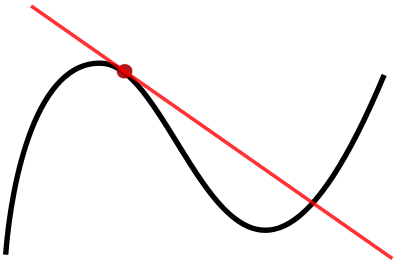
\includegraphics[width=.5\linewidth]{figures/NumericalAndMath/400px-Tangent_to_a_curve.png}
\end{center}
\caption{The graph of a function, drawn in black, and a tangent line to that function, drawn in red. The slope of the tangent line is equal to the derivative of the function at the marked point. (Text from \url{https://en.wikipedia.org/wiki/Derivative} on 2015.05.07; borrowing it because I couldn't find a better way to say it!)}
\end{figure}

\todo{Create a better figure for derivative definition and finite difference, with shown $\Delta x$}

\subsection{Integrals}

Integration 
An indefinite integral 



\begin{equation}
\int_a^b \! f(x)\,dx = F(b) - F(a)
\end{equation}

\begin{equation}
\int_a^b \! f(x)\,dx
\end{equation}

\begin{figure}[!ht]
\begin{center}
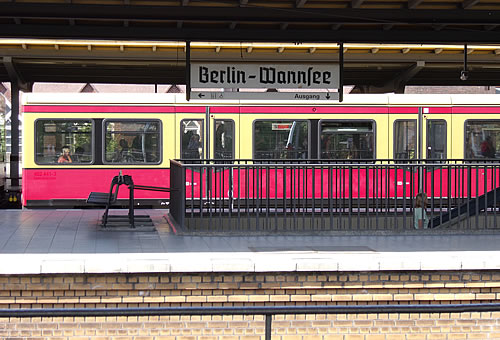
\includegraphics[width=.5\linewidth]{figures/NumericalAndMath/BerlinWannsee.jpg}
\end{center}
\caption{This ``S'' in the Berlin--Wannsee station sign is written in the old style. It is used for integrals to stand for ``sum'', as the area under a curve can be imagined to be a sum $\left( \sum \right)$ of every infinitessimally thin column of space under a curve.}
\end{figure}

\begin{figure}[!ht]
\begin{center}
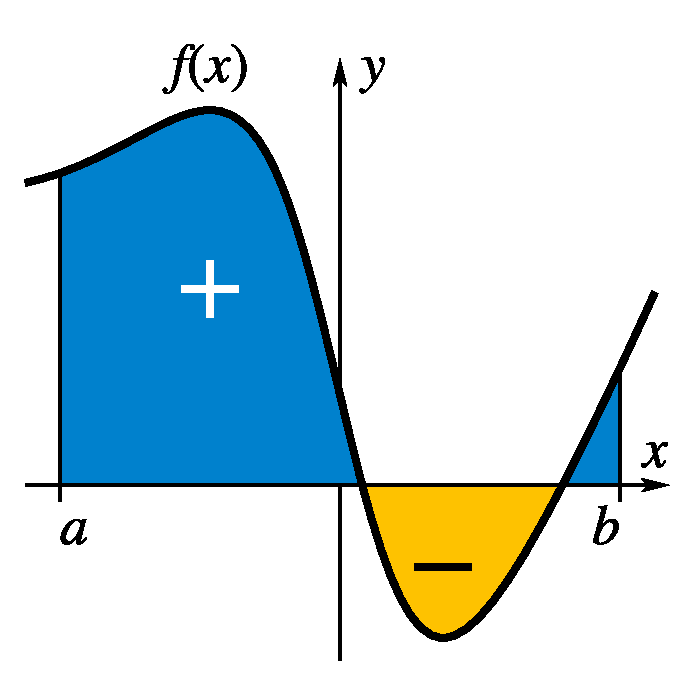
\includegraphics[width=.5\linewidth]{figures/NumericalAndMath/IntegralExample.pdf}
\end{center}
\caption{An integral is the sum of all area under a curve. (Contributed to Wikimedia Commons by User:KSmrq)}
\end{figure}

\subsection{Taylor series}

The Taylor series of any complex function $f(x)$ (i.e., $f(x) \in \mathbb{C}$) that is infinitely differentiable at a point $x_0$ approximates that function as a power series:
\begin{equation}
f(x_0)+\frac {f'(x_0)}{1!} (x-x_0)+ \frac{f''(x_0)}{2!} (x-x_0)^2+\frac{f^{(3)}(x_0)}{3!}(x-x_0)^3+ \cdots
\end{equation}
Or, in the more-compact summation notation, this is:
\begin{equation}
\sum_{n=0} ^ {\infty} \frac {f^{(n)}(x_0)}{n!} \, (x-x_0)^{n}
\end{equation}
where $n$ is the number of the derivative of $f$.

\begin{figure}[!ht]
\begin{center}
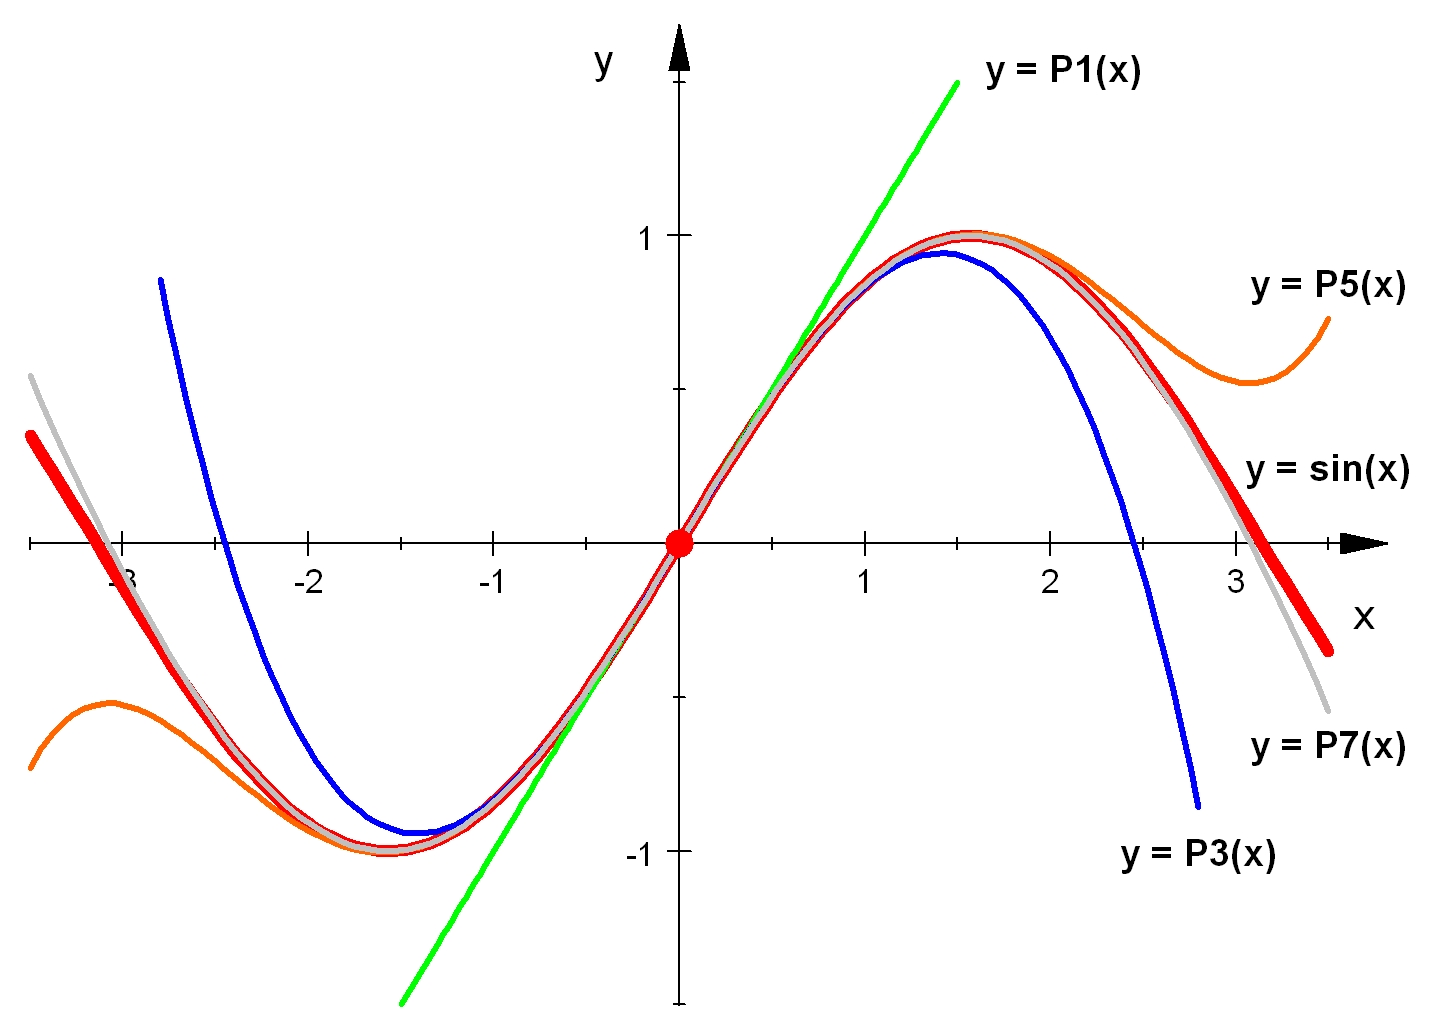
\includegraphics[width=.8\linewidth]{figures/NumericalAndMath/Taylor_Approximation_of_sin(x).jpeg}
\end{center}
\caption{Increasing orders of the derivative $n$, denoted P$n$, where $n = 1, 2, 3, \cdots$, show the increasing approximation of a sum of polynomials to the sine function.}
\end{figure}

\section{Finite difference}

One of the most useful functions of computers is their ability to approximate the values of derivatives at points. This allow us to directly compute approximations of the values of derivatives in differential equations and therefore solve them, typically through space and/or time.

You may have wondered why I covered derivatives and Taylor series right after one another. This is because these provide two ways to generate finite difference solutions to differential equations. The definition of a derivative provides a way to think of a derivative as the linear tangent to a curve at a given point -- and hence, also, to be well-approximated by a straight line over a finite distance so long as that distance is small compared to the nonlinearity of the curve that it is approximating. The Taylor series provides a less-visual but more powerful way to consider higher-order equations that could fit a curve near a certain point.

The result of this section will be a formalilzation of the \textbf{finite difference method}, by which a set of differential equations is estimated on a grid with constant spacings between grid cells (hence finite difference) and then solved. To provide a bit more background, finite difference is just one of several major methods for modeling with continuum equations. Other methods are finite volume (similar to finite difference except considering full cell volume, finite element (which allows a more irregular grid) and spectral (using how something varies in terms of periodic functions in order to write solutions to equations). Agent-based models that follow the actions of individual ``agets'' in a computational space also exist. These agents are often given simple rules and then allowed to interact with one another.

\subsection{Thermal diffusion}

In the example given here, we will solve the diffusion equation. First, I will present a derivation.

Heat is conducted at a rate that is proportional to the:
\begin{itemize}
 \item \textbf{Temperature difference (directly proportional)}: hotter things more quickly make other things hotter and colder things more quickly make other things colder. The contents of a bottle placed in the freezer will become cold more quickly than will those of one placed in the refrigerator
 \item \textbf{Distance along which heat must be conducted (inversely proportional)}: if there is a thicker wall to a thermos, cooler, or refrigerator, it will better insulate the heat
\end{itemize}
The constant of proportionality, $k$, is called the ``thermal conductivity'' and tells one how easily heat is conducted through a medium. It is an analog to electrical conductivity.

Putting all of these together, we can write (in one dimension):
\begin{equation}
 q_x = k \frac{d T}{d x}
\end{equation}
Here, $q_x$ is the heat flux (units of Watts per meter squared [W m$^{-2}$]).

This can be paired with an expression that relates heat flux to change in temperature. As one might expect, temperature increases with heat flux in and decreases with heat flux out. So it is the negative spatial derivative of heat flux that provides the negative divergence (i.e. convergence) of heat at the point of interest. Assuming no phase changes (e.g., solid to liquid), this occurrs at a rate that is inversely proportional to the heat capacity of the material. This is given by the specific heat capacity, here given assuming constant pressure ($c_p$), times the density ($\rho$). Given again in one dimension:
\begin{equation}
 \frac{\partial T}{\partial t} = -\frac{1}{c_p \rho} \frac{\partial q_x}{\partial dx}
\end{equation}

Putting these two equations together yields the \emph{diffusion equation}, one of the most widely-used equations in science.
\begin{equation}
 \frac{\partial T}{\partial t} = -\frac{k}{c_p \rho} \frac{\partial^2 q_x}{\partial dx^2}
\end{equation}
Redefining the coefficients on the right-hand side of the equation as $\kappa$ yields:
\begin{equation}
 \frac{\partial T}{\partial t} = -\kappa \frac{\partial^2 q_x}{\partial dx^2}
\end{equation}
This can be used to model chemical fluxes, temperature fluxes, hillslope change, and many more processes.

\subsection{Discretization}





Forward difference and ``implicit''
on both structured and unstructured meshes

Stencils

Linearizing equations (is this the right word? turning them into a set of linear equations)

Differential equations and linear algebra review

Include examples

\end{document}          
